\documentclass[11pt,a4paper]{scrartcl}

% Setup document
% Import Eidesstattliche Erklärung
\usepackage{pdfpages}
% Import graphics and wrap them
\usepackage{graphicx}
\usepackage{wrapfig}
\usepackage{float}

% Localization
\usepackage[utf8]{inputenc}
\usepackage[T1]{fontenc}
\usepackage[ngerman]{babel}

% Clickable table of contents
\usepackage{hyperref}
\usepackage[ngerman]{cleveref}

% Page formatting
\usepackage[automark]{scrlayer-scrpage}
\usepackage{typearea}
\usepackage{microtype}

% Better tables
\usepackage{tabularray}
\usepackage{booktabs}

% Develop Packages
\usepackage{blindtext}
% Variables
\newcommand{\vorname}{Lukas}
\newcommand{\nachname}{Szimtenings}
\newcommand{\matr}{Matr.-Nr.\ 3217694}
\newcommand{\uni}{FH Aachen}
\newcommand{\studiengang}{Angewandte Mathematik und Informatik}
\newcommand{\modul}{5. Semester 952006 (Aachen)}
\newcommand{\erstpruefer}{Alexander Voß}
\newcommand{\zweitpruefer}{Raphael Majeed}
\newcommand{\subtitel}{ Verteilte Ausführung von in konjunktiver Normalform spezifizierten Machbarkeitsabfragen in medizinischen Datenintegrationszentren }
\newcommand{\titel}{- Seminararbeit -}
\newcommand{\location}{Aachen}
\newcommand{\abteilung}{Abteilung: Research Infrastructure}
\newcommand{\abteilungabkuerzung}{RI}

%images
\newcommand{\uklogo}{
    
\includegraphics[scale=0.5]{res/logo-uniklinik-rwth-aachen}
    
\includegraphics[scale=0.6]{res/imi_sublogo}
}

\newcommand{\ukimilogo}{
\includegraphics[scale=0.16]{res/imilogo}}
% command for wrapfigure -> more than one figure per paragraph
\newcommand*{\invisiblepar}{{\setlength{\parfillskip}{0pt}\par}\vskip-\parskip\noindent\ignorespaces}
% Metadata
\title{\titel}
\author{\vorname{} \nachname}
\date{\today{}, \location}

% Pagestructure
\clearpairofpagestyles
%footer
\ifoot[]{\ukimilogo}
\cfoot[]{\abteilungabkuerzung}
\ofoot[]{\pagemark}
%header
\ihead[]{\vorname\ \nachname}
\chead[]{\titel}
\ohead[]{\matr}
%Seperator
\setheadsepline[\textwidth]{1pt}
\setfootsepline[\textwidth]{1pt}

\begin{document}
%% Prefix %%
% Titelblatt
\begin{titlepage}
    \centering
    {\scshape\LARGE \uni{} \par \studiengang{} \par \modul{} \par}
    \vspace{1cm}
    {\scshape\Large \titel{} \par}
    \vspace{1.5cm}
    {\bfseries \huge \subtitel{} \par}
    \vspace{2cm}
    {\Large \vorname{} \nachname{} \par \matr{} \par}
    \vfill
    \begin{center}
        \itclogo{}
        \par
        \abteilung{}
    \end{center}

    \par\vfill
    \parbox{4cm}{\hrule \strut{} \centering \footnotesize \vorname{} \nachname{} \par \textit{Autor}}
    \hfill
    \parbox{5cm}{\hrule \strut{} \centering \footnotesize \erstpruefer{} \par \textit{Erstprüfer}}
    \hfill
    \parbox{4cm}{\hrule \strut{} \centering \footnotesize \zweitpruefer{} \par \textit{Zweitprüfer}}
    \vfill
    {\large \location{} \today \par}
\end{titlepage}
% Einbinden der Eidesstattlichen Erklärung
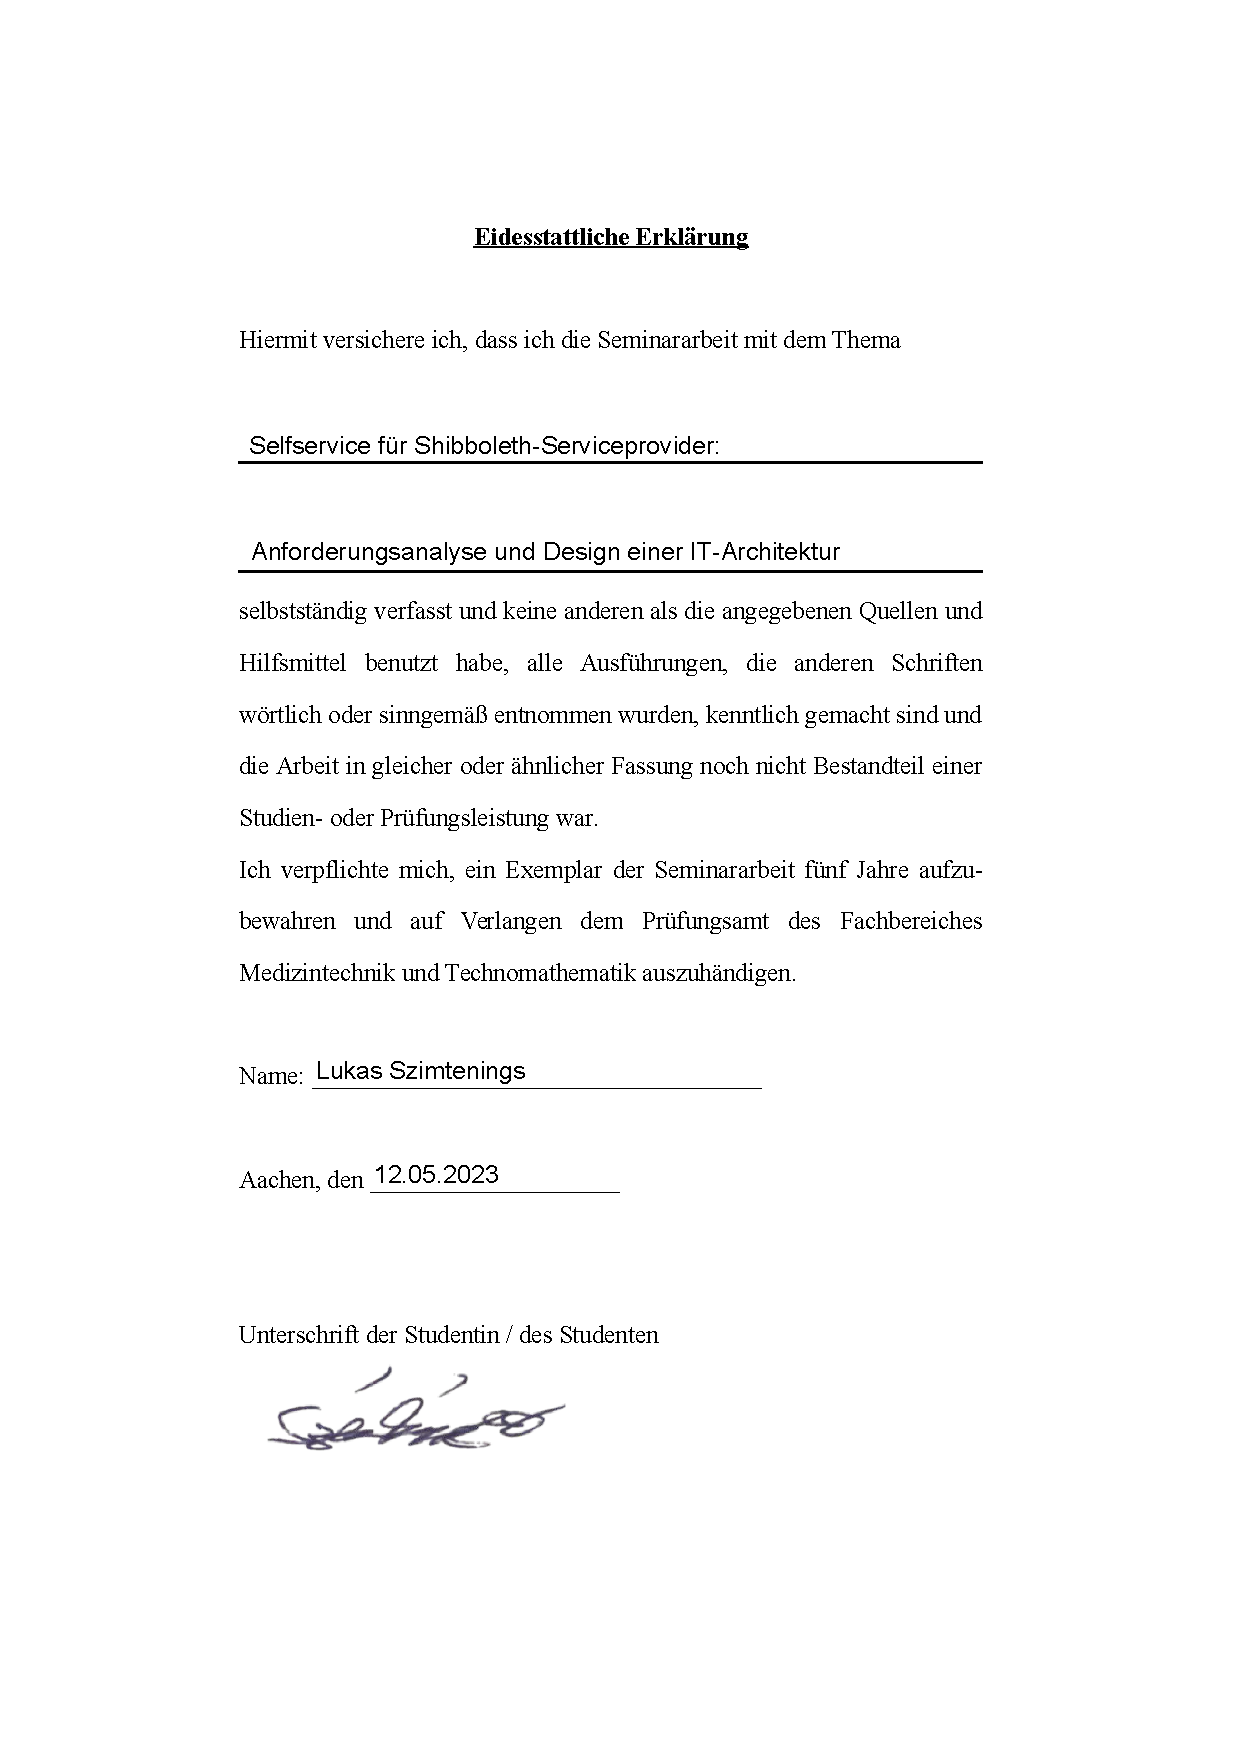
\includepdf{res/EidesstattlicheErklaerung.pdf}
\tableofcontents
\newpage

%% Hauptteil %%
% Seitenzahlen beginnen ab hier
\pagenumbering{arabic}

\section{Einführung}\label{sec:einfuehrung}
Die zunehmende Digitalisierung in Unternehmen führt dazu, dass Prozesse immer mehr automatisiert werden müssen, um wettbewerbsfähig zu bleiben.
Dabei stellt insbesondere die Verwaltung von Zugriffsberechtigungen eine Herausforderung dar, da diese oft sehr komplex und zeitaufwändig ist.
Eine Möglichkeit Zugriffsberechtigungen auf Systeme einer ganzen Organisation und darüber hinweg föderiert zu verwalten ist die Nutzung eines Single Sign-On (SSO) Systems.
Die RWTH Aachen verwendet bereits ein solches System, musste jedoch feststellen, dass durch die Verwaltung von Serviceprovidern ein nicht geringer administrativer Aufwand anfällt.
Zur Entwicklung eines Self-Service Systems muss daher zunächst die Verwaltung von Serviceprovidern auf der Prozessebene analysiert werden.

\subsection{Problemstellung}\label{subsec:problemstellung}
Ein SSO System besteht in aller Regel aus mindestens zwei Komponenten, zum einen dem Identity Provider (IDP) welcher konzeptionell Nutzer authentifiziert und autorisiert, und dem Service Provider (SP) welcher auf Basis der Informationen vom IDP über den Nutzer Zugriff auf seine Ressourcen gewährt.
Das von der RWTH betriebene Shibboleth ist ein solches System, welches vielseitigen Einsatz an der RWTH und übergeordneten Organisationen findet.
Da aus Sicherheitsgründen nicht jeder SP Zugriff auf das SSO System erhalten soll, muss die Verwaltung von SPs zentral in der Hand des IDPs liegen.
Dies führt jedoch zu einem hohen Verwaltungsaufwand, da die Anzahl der SPs stetig wächst und die Verwaltung der Zugriffsberechtigungen für jeden SP händisch in der IDP Konfiguration erfolgt.
Da die Konfigurationsdatei eine Sicherheitsrelevante Resource darstellt, ist die Anzahl der Personen die diese bearbeiten dürfen begrenzt.

\subsection{Zielsetzung}\label{subsec:zielsetzung}
Ziel dieser Seminararbeit ist es daher, die Verwaltung von SPs auf der Prozessebene zu analysieren und zu modelieren.
In einer Anforderungsanalyse soll dann erarbeitet werden, welche Anforderungen ein Self-Service System erfüllen muss um möglichst viele Teilprozesse an SP Betreiber auszulagern.
\subsection{Abgrenzung}\label{subsec:abgrenzung}
Nicht Ziel dieser Arbeit ist es, ein Systementwurf oder gar Code zu erstellen.
Es soll lediglich eine Analyse der Prozesse erfolgen, und auf Basis dieser eine Anforderungsanalyse durchgeführt werden.

\section{Grundlagen}\label{sec:grundlagen}
Erklärung der Begriffe, Theorie dahinter und dem State of the art
\subsection{Prozessanalyse}\label{subsec:prozessanalyse-grundlagen}
Die Identifikation und Abbildung von Geschäftsprozessen ist ein wichtiger Schritt, um die Effektivität und Effizienz von Unternehmen zu verbessern.
Durch die Abbildung von Prozessen können Schwachstellen und Engpässe erkannt und optimiert werden.
Im Laufe der Jahre wurden verschiedene Methoden und Modelle zur Prozessidentifikation und -abbildung entwickelt.
Im Folgenden werden einige der bekanntesten und erfolgreichsten Ansätze vorgestellt:

\subsubsection{UML}
Die Unified Modeling Language (UML) ist ein Standard für grafische Modellierung die für die Softwareentwicklung und das Systemdesign entwickelt wurde und die Darstellung und Dokumentation der Struktur und des Verhaltens von Systemen ermöglicht (OMG, 2021).
Im Zusammenhang mit der Prozessmodellierung können im speziellen Aktivitätsdiagramme verwendet werden, um Prozesse in Aktionen aufgeteilt darzustellen, wobei verschiedene Akteure durch Swimlanes repräsentiert werden können \cite{List2006}.\\

Allerdings hat die UML bei der Modellierung von Geschäftsprozessen gewisse Einschränkungen.
Während sie umfassende Unterstützung für Kontrollfluss- und Datenperspektiven bietet, ist ihre Anwendbarkeit auf ressourcenbezogene oder organisatorische Aspekte begrenzt (Russell et al., 2006).
Darüber hinaus kann UML Schwierigkeiten haben, einige natürliche Konstrukte zu erfassen, die in Geschäftsprozessen vorkommen, wie z. B. Fälle und Interaktionen mit der betrieblichen Umgebung (Russell et al., 2006).
Folglich sind spezialisierte Sprachen wie Business Process Model and Notation (BPMN) aufgrund ihrer expliziten Ausrichtung auf prozessspezifische Konstrukte und Notationen möglicherweise besser für die Geschäftsprozessmodellierung geeignet (Chinosi \& Trombetta, 2012).

\subsubsection{BPMN (Business Process Model and Notation)}

BPMN ist ein international anerkannter Standard zur Modellierung von Geschäftsprozessen.
Es ist eine grafische Notation, die es erlaubt, Geschäftsprozesse auf eine visuelle und leicht verständliche Art darzustellen.
BPMN wird häufig eingesetzt, da es die Möglichkeit bietet, die Zusammenhänge zwischen Aktivitäten, Entscheidungen und Prozessflüssen einfach und übersichtlich abzubilden.
Darüber hinaus erlaubt BPMN die Integration mit anderen Business-Systemen und ist somit ein beliebtes Werkzeug zur Analyse und Optimierung von Geschäftsprozessen.

\subsubsection{Event-driven Process Chain (EPC)}

EPC ist ein Prozessmodellierungskonzept, das auf der Idee basiert, dass Prozesse aus einer Reihe von Ereignissen und Funktionen bestehen.
EPCs bieten eine grafische Darstellung, die es erlaubt, den Prozessfluss auf eine visuelle und verständliche Art darzustellen.
Die Methode wird häufig eingesetzt, da sie es ermöglicht, die Abhängigkeiten zwischen Prozessschritten einfach abzubilden und somit die Identifikation von Engpässen und Schwachstellen zu erleichtern.

\subsubsection{Value Stream Mapping (VSM)}

VSM ist eine Methode, die in der Produktion eingesetzt wird, um den Wertstrom zu visualisieren und zu verbessern.
Es ist jedoch auch für die Identifikation und Optimierung von Geschäftsprozessen geeignet.
VSM bietet eine grafische Darstellung, die es ermöglicht, den Fluss von Material und Informationen durch den Prozess zu visualisieren.
Die Methode ist besonders effektiv bei der Identifikation von Verschwendung und der Optimierung von Engpässen.

\subsubsection{Lean Six Sigma}

Lean Six Sigma ist eine Kombination aus den beiden Managementmethoden Lean Manufacturing und Six Sigma.
Es wird oft als Prozessverbesserungsansatz verwendet, um die Qualität von Produkten und Dienstleistungen zu verbessern, die Kundenzufriedenheit zu erhöhen und die Effizienz von Prozessen zu steigern.
Lean Six Sigma nutzt eine Daten-getriebene Methode zur Identifikation und Beseitigung von Fehlern, Reduktion von Variabilität und Optimierung von Prozessen.\\

Die Methode basiert auf fünf Phasen: Define, Measure, Analyze, Improve und Control (DMAIC).
In der Define-Phase werden die Ziele des Projekts und die Kundenerwartungen definiert.
In der Measure-Phase werden Prozesskennzahlen ermittelt, um den aktuellen Zustand zu messen.
In der Analyze-Phase werden Ursachen für Probleme und Schwachstellen identifiziert.
In der Improve-Phase werden Maßnahmen zur Beseitigung von Schwachstellen und zur Verbesserung der Prozesse entwickelt.
In der Control-Phase werden Prozesse stabilisiert und kontrolliert, um sicherzustellen, dass die Verbesserungen nachhaltig sind.\\

Vorteile von Lean Six Sigma sind unter anderem eine höhere Kundenzufriedenheit, höhere Qualität, gesteigerte Effizienz und geringere Kosten.
Die Methode fördert auch eine kundenorientierte Denkweise und eine kontinuierliche Verbesserung der Prozesse.
Allerdings erfordert die Implementierung von Lean Six Sigma oft eine umfassende Schulung und eine hohe Beteiligung des Personals, um die Methode effektiv anwenden zu können.\\

Ein Nachteil von Lean Six Sigma kann sein, dass es sehr datengetrieben ist und manchmal vernachlässigt, dass auch Erfahrung und Intuition wichtige Faktoren für die Prozessoptimierung sein können.
Außerdem kann die Implementierung von Lean Six Sigma in manchen Unternehmen aufgrund von Widerständen und fehlender Unterstützung der Führungsebene schwierig sein.\\

\subsubsection{Conclusion}

Die in diesem Kapitel vorgestellten Methoden und Modelle zur Prozessidentifikation und -abbildung bieten verschiedene Ansätze und Werkzeuge zur Analyse und Optimierung von Geschäftsprozessen. Die Auswahl der Methode hängt dabei von verschiedenen Faktoren ab, wie zum Beispiel dem Zweck der Analyse, der Komplexität des zu untersuchenden Prozesses oder der verfügbaren Ressourcen.

Die BPMN 2.0 ist eine weit verbreitete und standardisierte Notation zur Modellierung von Geschäftsprozessen. Sie ermöglicht eine klare und einheitliche Darstellung von Prozessen und bietet zahlreiche Möglichkeiten zur Analyse und Optimierung. Allerdings ist sie aufgrund ihrer Komplexität nicht immer einfach zu handhaben und erfordert eine umfassende Einarbeitung.

Die Event-driven Process Chain (EPC) ist eine Methode zur Modellierung von Geschäftsprozessen, die sich insbesondere für komplexe Prozesse eignet. Sie bietet eine klare und präzise Darstellung der Prozesse und ermöglicht es, Schwachstellen und Engpässe zu identifizieren.

Die IDEF0 Methode bietet eine strukturierte und detaillierte Modellierung von Prozessen und ist besonders für komplexe Prozesse geeignet. Allerdings ist sie aufgrund ihrer Formalisierung und Notation nicht immer intuitiv und erfordert ebenfalls eine umfassende Einarbeitung.

Die Value Stream Mapping Methode ist besonders geeignet, um den Material- und Informationsfluss in Prozessen zu visualisieren und zu optimieren. Dabei wird besonderer Wert auf die Eliminierung von Verschwendungen gelegt. Die Methode ist schnell erlernbar und einfach anwendbar, jedoch nicht immer geeignet für komplexe Prozesse.

Insgesamt bieten die vorgestellten Methoden und Modelle verschiedene Ansätze zur Analyse und Optimierung von Geschäftsprozessen. Es empfiehlt sich, die spezifischen Anforderungen und Ziele der Prozessanalyse zu berücksichtigen, um die passende Methode auszuwählen.


\begin{longtblr}{
    vlines, hlines,
    colspec={X[m,c]X[c]X[c]X[c]},
    rowhead=1,
    }
    & \textbf{Event-driven process chain} & \textbf{Lean six sigma} & \textbf{Value Stream Mapping} \\
    \textbf{Anwendungsgebiet} & komplexe Prozesse und Abläufe mit vielen Abhängigkeiten und Entscheidungen. & Optimierung von Produktionsprozessen in der Industrie. & Verbesserung von Material- und Informationsflüsse in Produktionsprozessen. \\
    \textbf{Ziel} & Identifikation von Flaschenhälsen und Engpässen & Reduzierung von Fehlern und Variationen in Produktionsprozessen & Identifikation von Verschwendungen in der Wertschöpfungskette \\
    \textbf{Schwerpunkt} & Fokussiert auf die Analyse der Prozesslogik und Identifikation von Abhängigkeiten und Entscheidungen. & Fokussiert auf die Reduktion von Prozessvariationen und -fehlern. & Fokussiert auf die Optimierung von Material- und Informationsflüssen durch die Identifikation und Beseitigung von Verschwendungen. \\
    \textbf{Vorteile} & Ermöglicht eine detaillierte Analyse der Prozesslogik und ermöglicht eine schnelle Identifikation von Flaschenhälsen und Engpässen. & Betont die systematische Reduktion von Prozessvariationen und -fehlern und liefert dadurch langfristige und nachhaltige Prozessverbesserungen. & Ermöglicht eine schnelle Identifikation von Verschwendungen und deren Beseitigung, was zu einer Verbesserung der Material- und Informationsflüsse und einer Reduktion von Aufwänden führt. \\
    \textbf{Nachteile} & Kann bei sehr einfachen Prozessen überdimensioniert und zu komplex sein. & Fokussiert stark auf die Reduktion von Fehlern und Variationen, was zu einer Vernachlässigung anderer Aspekte der Prozessoptimierung führen kann. & Kann zu einer Vernachlässigung von Prozessverbesserungen in anderen Bereichen außerhalb der Wertschöpfungskette führen. \\
\end{longtblr}

Erklärung von Prozessanalyse, verschiedenen Methoden und Modellen
\subsection{Anforderungsanalyse}\label{subsec:anforderungsanalyse-grundlagen}
Erläuterung des Begriffs Anforderungsanalyse aufzeigen verschiedener Methoden und Modellierungstechniken 

\section{Methodik}\label{sec:methodik}
Hier erkläre ich warum ich welche der oben genannten Methoden gewählt habe und wie ich sie im Detail angewandt habe
\subsection{Prozessanalyse}\label{subsec:prozessanalyse-methodik}
Die Methodik zur Prozessanalyse dieser Seminararbeit bezieht sich in großen Teilen auf den Define Teil von Lean Six Sigma.
Vorteile gegenüber den anderen in Kapitel \ref{sec:prozessanalyse-grundlagen} vorgestellten Methoden und Modellen werden im folgenden diskutiert.
Verglichen mit EPC bietet Lean Six Sigma einen standardisierten Prozess zur Analyse und Optimierung von Prozessen, während EPC mehr die Modellierungsebene bedient.
Im Vergleich zu Value Stream Mapping (VSM) betont Lean Six Sigma ebenfalls die statistische Analyse von Prozessdaten und die Reduzierung von Variationen, während VSM sich eher auf die Identifikation von Verschwendungen und die Verbesserung von Material- und Informationsflüssen konzentriert. VSM bietet jedoch eine bessere Unterstützung für die Analyse von Wertschöpfungsketten und die Identifikation von Engpässen. Insgesamt ist Lean Six Sigma jedoch besser geeignet, um spezifische Prozessprobleme zu identifizieren und zu beheben.

Ein weiterer Vergleich kann mit der Theory of Constraints (ToC) gezogen werden, die sich ebenfalls auf die Identifikation von Engpässen und Flaschenhälsen in Prozessen konzentriert. ToC bietet jedoch eine umfassendere Methodik zur Identifikation und Beseitigung von Engpässen, während Lean Six Sigma eher auf die Reduzierung von Fehlern und Variationen fokussiert ist. Insgesamt kann ToC jedoch als eine erweiterte Version von Lean Six Sigma betrachtet werden, da es Lean-Prinzipien integriert und zusätzlich eine umfassendere Methodik bietet.

Zusammenfassend lässt sich sagen, dass Lean Six Sigma eine effektive Methode zur Optimierung von Prozessen und Produktionsprozessen ist, die insbesondere durch ihre statistische Analysefähigkeit und den Fokus auf die Reduktion von Fehlern und Variationen gekennzeichnet ist. Im Vergleich zu anderen Methoden kann es jedoch weniger flexibel sein und bestimmte Aspekte der Prozessoptimierung vernachlässigen.
Erklärung warum ich welche Methodik gewählt habe, und wie ich sie angewandt habe
\subsubsection{Entwurf des Fragenkatalogs}\label{subsubsec:entwurf-fragenkatalog}
Wie habe ich meinen Fragenkatalog entworfen, und welche Fragen habe ich gestellt
\subsubsection{Auswahl der Gesprächspartner}\label{subsubsec:auswahl-gespraechspartner}
Wie habe ich die Gesprächspartner ausgewählt, und nach welcher Methodik bin ich bei der Befragung vorgegangen
\subsection{Anforderungsanalyse}\label{subsec:anforderungsanalyse-methodik}
Weiß noch nicht was hier hin soll, aktuell nur für Symmetrie hier

\section{Ergebnisse und Diskussion}\label{sec:results}
\subsection{Prozessanalyse}\label{subsec:prozessanalyse-results}
\subsubsection{Ergebnisse}\label{subsubsec:prozessanalyse-results}
Ergebnisse bestehend aus zunächst den Fragen und Antworten, und dann dem daraus resultierenden Modell des Prozesses
\subsubsection{Diskussion}\label{subsubsec:prozessanalyse-discussion}
Diskussion der Ergebnisse, eventueller Schwächen im Prozess und Verbesserungsvorschläge
\subsection{Anforderungsanalyse}\label{subsec:anforderungsanalyse-results}
Auflistung der erarbeiteten Anforderungen eingeteilt in funktionale und nicht funktionale Anforderungen
\subsubsection{Funktionale Anforderungen}\label{subsubsec:functional-requirements}
\subsubsection{Nicht-funktionale Anforderungen}\label{subsubsec:non-functional-requirements}
\subsubsection{Diskussion}\label{subsubsec:anforderungsanalyse-discussion}

\section{Zusammenfassung und Ausblick}\label{sec:summary}
\subsection{Zusammenfassung}\label{subsec:summary}
\subsection{Ausblick}\label{subsec:outlook}

%% Suffix %%
\newpage

% Bibliographie
\pagenumbering{Roman}
\bibliography{Seminararbeit}
\bibliographystyle{unsrt}

% Abbildungsverzeichnis
\listoffigures
\end{document}